\documentclass{beamer}
\usepackage{graphicx}
\usepackage{multicol}
\usepackage{setspace}
\usepackage{xcolor}
\usepackage{xy}
\usepackage{xypic}

\usepackage[strict]{changepage}

\newcommand{\fullwidth}[1]{\noindent\checkoddpage\makebox[0pt][r]{\makebox[\dimexpr1in+\hoffset+\ifoddpage\oddsidemargin\else\evensidemargin\fi][l]{#1}}}
\newcommand{\truecenter}[1]{\fullwidth{\parbox[c]{\paperwidth}{#1}}}

\setstretch{1.3}

\def\untrusted#1{\save[].[#1]*[F]\frm{}\restore}
\def\trusted#1{\save[].[#1]*[F=]\frm{}\restore}


\begin{document}
\title{Coq Framework for security policies and proof of concept application}
\author{Anders Kaseorg, Jason Gross, and Peng Wang} 
\date{December 10, 2014 \\ 6.858 --- Fall 2014} 

\frame{\titlepage} 

\begin{frame}{\Huge The Problem}
\Large
\begin{multicols}{2}
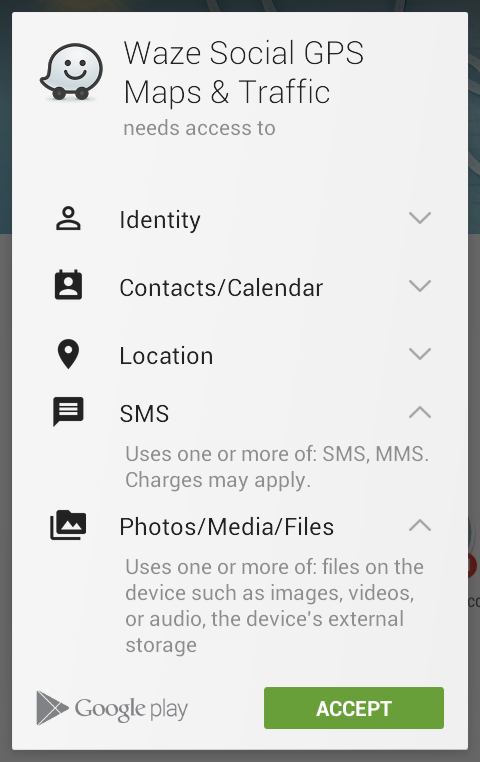
\includegraphics[height=0.75\textheight]{waze}
\columnbreak
\begin{itemize}
  \item Fixed set of coarse permissions
  \item No information flow control
% notes: what if we want to say that the app isn't allowed to send embarassing pictures to anyone without my permission?  Or that it's not allowed to eat too much CPU or battery?
\end{itemize}
\end{multicols}
\end{frame}

\begin{frame}{\Huge Our Idea}
\Large
\begin{itemize}
  \item Design expressive language allowing:
  \begin{itemize}\Large
    \item enforcement of fine-grained security policies
    \item little to no runtime overhead \pause
    \item correctness proofs \small (everything is better with more proofs!)
  \end{itemize}
\end{itemize}
\end{frame}



\begin{frame}{\Huge Our Project: A Proof of Concept}
\Large
\begin{itemize}
  \item Framework \& Password Manager
  \item Implemented in Coq 
\includegraphics[width=0.05\textwidth]{coq-logo}
  \item Based on compile-time enforced modularity and parametricity
  \item Demo: \url{https://andersk.scripts.mit.edu/pwmgr/demo}
\end{itemize}
\end{frame}



\begin{frame}{\Huge Example Specification}
\Large
\vspace{-0.2in}
\truecenter{%
\[
\xymatrix@-0.5pc{
&\trusted{ddddddrrrr} \\
&&\untrusted{dddd}\txt{\phantom{UI}}& \txt{\phantom{Encrypt}} & \untrusted{dddd}\txt{\phantom{Net}}&& \\
&&\txt{\phantom{UI}}\ar[r]& \trusted{}\txt{\textbf{Encrypt}}\ar[r]     &                 \txt{\phantom{Net}}\ar@{=>}[rrr]^>{\txt{Network Out}}&&& \\
\ar@{=>}[rr]^<{\txt{User In\ \ \phantom{.}}}&&\txt{UI}&  \ar[u]\ar[d]\trusted{}\txt{\textbf{Secret Key}}     &                 \txt{Net}& \\
&&\txt{\phantom{UI}}&  \ar[l]\untrusted{}\txt{Decrypt}     & \ar[l] \txt{\phantom{Net}}&&&\ar@{=>}[lll]^<{\txt{Network In}} \\
&&\txt{\phantom{UI}}& \txt{\phantom{Encrypt}} & \txt{\phantom{Net}}&& \\
&&\txt{\phantom{UI}}& \txt{\phantom{Encrypt}} & \txt{\phantom{Net}}&& \\
}
\]
}
\end{frame}


\begin{frame}{\Huge Future Work}
\Large
\begin{itemize}
  \item termination proofs $\longrightarrow$ absolute running time
  \begin{itemize}\large
    \item lack of timing side-channels in the presence of malicious untrusted code
    \item currently, we only handle timing side-channels under the assumption of quick code
  \end{itemize}
  \item more modular termination / timing proofs
  \item more applications
\end{itemize}
\end{frame}

%\begin{frame}
  % demo, if time?
%\end{frame}

\end{document}